%!TEX root = guide2.0.tex

% \section{Summary}\label{sec:PyMCObjects}
Bayesian inference begins with specification of a probability model relating unknown variables to data. PyMC provides three basic building blocks for Bayesian probability models: \texttt{Stochastic}, \texttt{Functional} and \texttt{Potential}. 

A stoch object represents a variable whose value is not completely determined by its parents, and a functl object represents a variable that is determined by its parents. \texttt{Stochastic} and \texttt{Functional} are subclasses of \texttt{Variable}.

The third basic class, representing `factor potentials' (\cite{dawidmarkov,jordangraphical}), represents an arbitrary log-probability term. This object lends PyMC a great deal of flexibility, but it should be used sparingly if possible. It is most useful in situations where the dependence relationships between variables are not specified, such as Markov random fields. \texttt{Potential} and \texttt{Variable} are subclasses of \texttt{Node}.

PyMC also provides container classes for stochs and functls to ease programming of certain dependency situations, such as when a particular variable depends on every element of a Markov chain.

These objects are meant to perform a small set of behaviors efficiently. As such, they have very limited awareness of the probability model in which they are embedded and no methods for updating their values in an MCMC loop conditional on the rest of the model. PyMC leaves this stoch updating functionality to the \texttt{StepMethod} class and model-level MCMC supervision to the \texttt{Sampler} class. These objects are described in chapter \ref{chap:modelfitting}. 

Declared probability models can be wrapped in the \texttt{Model} class, which is able to perform model-level tasks such as drawing directed acyclic graphs (\cite{dawidmarkov,jordangraphical}) and computing Bayes factors (\cite{gelman}) but has no fitting functionality. Objects responsible for fitting probability models, such as \texttt{Sampler}, are subclasses of \texttt{Model}.

\section{The \texttt{Variable} classes: \texttt{Stochastic} and \texttt{Functional}}
Consider the following dataset, which is a time series of recorded coal mining disasters in the UK from 1851 to 1962.
\begin{center}
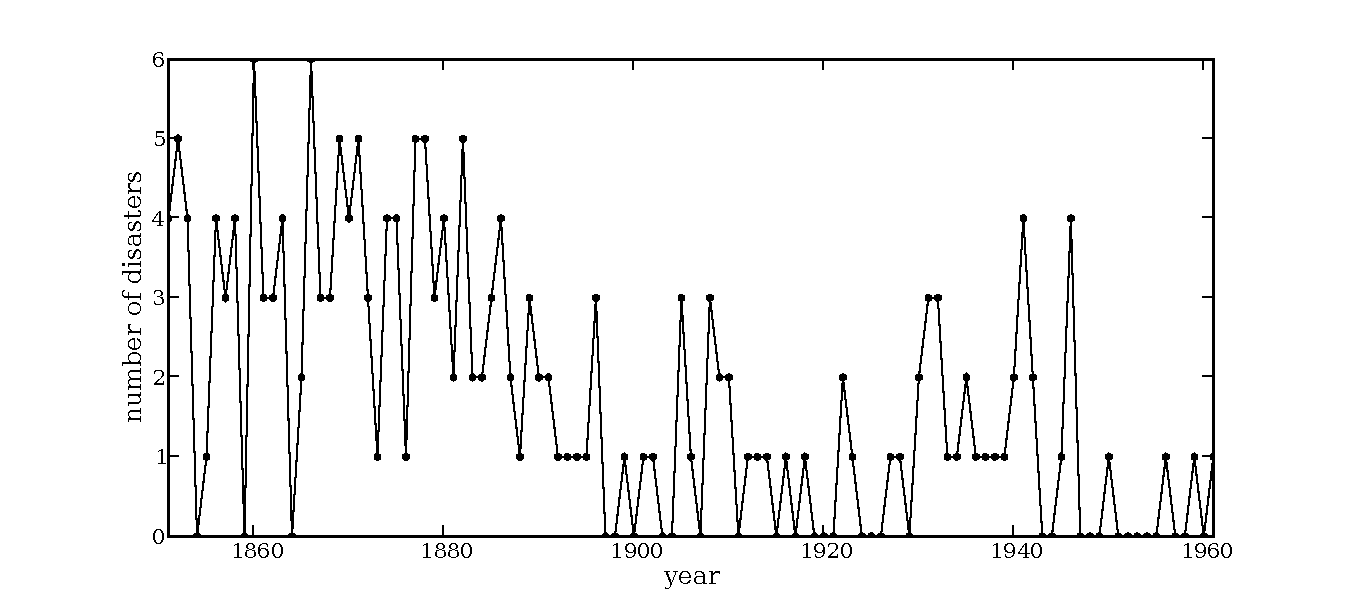
\epsfig{file=disasterts.pdf, width=15cm}
\end{center}
Occurrences of disasters in the time series is thought to be derived from a Poisson process with a large rate stoch in the early part of the time series, and from one with a smaller rate in the later part. We are interested in locating the change point in the series, which perhaps is related to changes in mining safety regulations.

We represent our conceptual model formally as a statistical model:
\begin{equation}
    \begin{array}{ccc}
        (D_t | s, e, l) \sim \textup{Po}\left(r_t\right), & r_t=\left\{\begin{array}{ll}
            e & t\le s\\ l & t>s
            \end{array}\right.,&t\in[t_l,t_h]\\
        s\sim \textup{U}(t_l, t_h)\\
        e\sim \textup{Exp}(r_e)\\
        l\sim \textup{Exp}(r_l)        
    \end{array}
    \label{disastermodel} 
\end{equation}
The symbols have the following meanings:
\begin{description}
    \item[$D_t$:] The number of disasters in year $t$.
    \item[$r_t$:] The rate stoch of the Poisson distribution of disasters in year $t$.
    \item[$s$:] The year in which the rate stoch changes.
    \item[$e$:] The rate stoch before the switchpoint $s$.
    \item[$l$:] The rate stoch after the switchpoint.
\end{description}
Because we have defined $D$ by its dependence on $s$, $e$ and $l$, the latter three are known as the \emph{parents} of $D$. $D$ is called the \emph{child} of $s$, $e$ and $l$. Similarly, parents of $s$ are $t_l$ and $t_h$, and $s$ is the child of $t_l$ and $t_h$.

At the model-specification stage (before the data have been observed), $D$, $s$, $e$, $r$ and $l$ are all \emph{random variables}. Under the Bayesian interpretation of probability, `random' variables are not necessarily believed to have arisen from a physical random process. `Random' only means that we are unsure of their values. Random variables are represented in PyMC by class \texttt{Variable}, which has subclasses \texttt{Stochastic} and \texttt{Functional}.

There is a difference between $r$ and the other variables: if we knew the values of $r$'s parents, we could compute the value of $r$ with no uncertainty. This variable is defined by a mathematical function which returns its value given values for its parents. 

On the other hand, even given values for the parents of $s$ we would still be uncertain of $s$'s value, and similarly for $D$, $e$ and $l$. These variables are defined by probability distributions that express how plausible their candidate values are given values for their parents.
 

\section{The \texttt{Stochastic} class}

In PyMC, variables of the latter type are represented by the \texttt{Stochastic} class and subclasses. A stoch has the following major attributes: 
\begin{description}
    \item[\texttt{value}:] Gives the stoch's current value.
    \item[\texttt{logp}:] Gives the log-probability of the stoch's current value given the values of its parents.
\end{description}
A stoch can optionally be endowed with a method called \texttt{\bfseries random}, which draws a value for the stoch given the values of its parents. Note that the \texttt{random} method does not provide a Gibbs sample unless the stoch has no children.

Stochastics expose the following additional attributes:
\begin{description}
    \item[\texttt{parents}:] A dictionary containing the stoch's parents. The keys of the dictionary correspond to the names assigned to the stoch's parents by the stoch, and the values correspond to the actual parents. For example, the keys of $s$'s parents dictionary would be \texttt{'t\_l'} and \texttt{'t\_h'}. Since PyMC inherits Python's dynamic typing, parents may be of any class or type.
    \item[\texttt{children}:] A set containing the stoch's children. This set is produced automatically; the user doesn't need to worry about filling it.
    \item[\texttt{isdata}:] A boolean indicating whether the stoch's value has been observed (is fixed).
    \item[\texttt{trace}:] The trace object assigned to the stoch, see chapter \ref{chap:database}.
    \item[\texttt{\_\_name\_\_}:] The name of the stoch, should be unique.
    \item[\texttt{\_\_doc\_\_}:] The docstring of the stoch.
\end{description}

Subclasses of \texttt{Stochastic} include the \texttt{DiscreteStochastic} class, which represents integer-valued variables, and the \texttt{BinaryStochastic} class, which represents Bernoulli or indicator variables. 

\subsection{Instantiation of stochs}
PyMC provides four ways to instantiate stochs, called the `short', `medium', `long' and `direct' interfaces.
\begin{description}
    \item[Short] \textbf{XXX}
    \item[Medium] Uniformly-distributed stoch $s$ could be instantiated using the medium interface as follows:
    \begin{verbatim}
@stochastic
def s(value=1900, t_l=1851, t_h=1962):
    """The switchpoint for the rate of disaster occurrence."""
    if value > t_h or value < t_l:
        return -Inf
    else:
        return -log(t_h - t_l) 
    \end{verbatim}
    The decorator \texttt{stoch} wraps the function \texttt{s} in a stoch object. This object will evaluate its log-probability using the function \texttt{s}. The \texttt{value} argument, which is required, provides an initial value for the variable. The names of the function's other arguments become the keys of the stoch's \texttt{parents} dictionary, which maps to the corresponding values (parent objects). The name of the function (in this case \texttt{s}) becomes the \texttt{\_\_name\_\_} of the stoch, and the docstring of the function is passed on to the stoch as well.

The stoch may be valued as any object, its parents may be any objects, and there is absolutely no restriction on the log-probability function, as long as it returns a \texttt{float}. Note that PyMC, scientific Python and numerical Python all provide fast implementations of several standard probability distributions that can be wrapped in stoch objects.

    The medium interface's decorator can take a flag called \texttt{trace} which signals to \texttt{Model} whether an MCMC trace should be kept for the stoch: \texttt{@stochastic(trace = False)} would turn tracing off.

    \item[Long] The long interface extends the medium interface by allowing the user to specify a \texttt{random} method for sampling the stoch's value conditional only on its parents.
    \begin{verbatim}
@stochastic
def s(value=1900, t_l=1851, t_h=1962):
    """The switchpoint for the rate of disaster occurrence."""

    def logp(value, t_l, t_h):
        if value > t_h or value < t_l:
            return -Inf
        else:
            return -log(t_h - t_l) 
            
    def random(t_l, t_h):
        return round( (t_l - t_h) * random() ) + t_l

    rseed = 1.
    \end{verbatim}
The stoch again gets its name, docstring and parents from function \texttt{s}, but in this case it will evaluate its log-probability using the \texttt{logp} function. The \texttt{random} function will be used when \texttt{s.random()} is called. Note that it doesn't take a \texttt{value} argument, because it provides a new value. \textbf{XXX David explain rseed} \texttt{rseed} provides a seed for the RNG. The \texttt{value} argument is optional if a \texttt{random} method is provided; if no initial value is provided, it will be drawn using the \texttt{random} method.

    \item[Direct] Some users may prefer not to use the \texttt{@stochastic} decorator, but to instantiate \texttt{Stochastic} directly:
\begin{verbatim}
def s_logp(value, t_l, t_h):
    if value > t_h or value < t_l:
        return -Inf
    else:
        return -log(t_h - t_l) 

def s_rand(t_l, t_h):
    return round( (t_l - t_h) * random() ) + t_l

s = Stochastic(logp = s_logp, 
name = 's', 
value = 1900,
parents = {'t_l': 1851, 't_h': 1962},
doc = 'The switchpoint for the rate of disaster occurrence.',
random = s_rand, 
trace = True, 
rseed = 1., 
isdata = False,
cache_depth = 2)
\end{verbatim}
\end{description}

\subsection{Don't update stochs' values in-place}\label{sub:warning}

\texttt{Stochastic} objects' values should not be updated in-place. This would confuse PyMC's caching scheme and destroy the `last value' attribute of the stoch, which is used for rejecting jumps. The only way a stoch's value should be updated is using statements of the following form:
\begin{verbatim}
    A.value = new_value
\end{verbatim}
where \texttt{new\_value} is an object that has just been created for this purpose. The following are in-place updates and should \emph{not} be used:
\begin{itemize}
    \item \texttt{A.value += 3}
    \item \texttt{A.value[2,1] = 5}
    \item \texttt{A.value.attribute = new_attribute_value}. This is an in-place update regardless of what type of object \texttt{A.value} is.
\end{itemize}

This restriction is not that bad. In Metropolis-Hastings-type step methods, the `current' and `proposed' values of a stoch must be stored simultaneously when evaluating a jump; if you were to update a stoch's value in-place in your own MCMC code, you would need to make a copy of its value beforehand. It does become onerous if a step method proposes values for the elements of an array-valued stoch separately. In this case, it may be preferable to divide the array-valued stoch into several stochs. See section \ref{sub:container}. 

\section{Data}

Although the data $D$ was a random variable at the model-specification stage, we subsequently fixed its value by observing it. In PyMC such variables are represented by \texttt{Stochastic} objects whose \texttt{isdata} attribute is set to \texttt{True}. If a stoch's \texttt{isdata} flag is \texttt{True}, its value cannot be changed.

\subsection{Why are data and unknown stochs represented by the same object?}
Since it's represented by a \texttt{Stochastic}, $D$ formally depends on $s$, $e$ and $l$ even though its value is fixed. This isn't just a quirk of PyMC's syntax; Bayesian hierarchical notation itself makes no distinction between unobserved random variables (stochs) and observed random variables (data). This point can be counterintuitive at first, as most scientists' instinct is to regard data as fixed a priori and unknown stochs' values as dependent on the data. The value of data is fixed, after all, so how could it depend on anything?

One way to understand this issue is to think of statistical models like (\ref{disastermodel}) as predictive models for data, or as models of the processes that gave rise to data. Before observing the value of $D$, we could have easily sampled from its prior predictive distribution $p(D)$ as follows:
\begin{enumerate}
    \item Sample $e$, $s$ and $l$ from their priors.
    \item Sample $D$ conditional on these values.
\end{enumerate}
Even after we observe the value of $D$, we need to use this process model to make inferences about $e$, $s$ and $l$.

\medskip
To look at the issue another way, we could in principle have written a model equivalent to (\ref{disastermodel}) in such a way that $D$ depended on nothing and everything else depended on $D$, for example
\begin{eqnarray*}
    s|e,l,D\sim\cdot\\
    e|l,D\sim\cdot\\
    l|D\sim\cdot\\
    D=D_*
\end{eqnarray*}

This would have felt more natural in some ways, because we would have the unknown stochs depending on the data. However, if we could write down that model using standard distributions we could trivially compute and sample from the posterior,
\begin{eqnarray*}
    p(s,e,l|D) = p(s|e, l, D) p(e|l, D) p(l|D),
\end{eqnarray*}
and we would have no use for MCMC or any other fitting method. Bayesian methods, and statistics in general, are needed when it's more natural to model the data as depending on the unknown stochs than vice versa.

\subsection{Declaring stochs to be data}

In the medium and long interfaces, a \texttt{Stochastic} object's \texttt{isdata} flag can be set to true by stacking a \texttt{@data} decorator on top of the \texttt{@stochastic} decorator:
\begin{verbatim}
@data
@stochastic
def D(value = count_array, switchpoint = s, early_rate = e, late_rate = l):
    """The observed annual disaster counts."""
    logp = sum(-value[:switchpoint]) + early_rate * log(value[:switchpoint]) \
            - gammaln(early_rate))
    logp += sum(-value[switchpoint:] + late_rate * log(value[switchpoint:]) \
            - gammaln(late_rate))
    return logp
\end{verbatim}
In the direct interface, the \texttt{isdata} argument can be simply set to \texttt{True}.


\section{The \texttt{Functional} class}\label{functl}

Functionals represent variables whose values are fully determined by the values of their parents. The variables on which a functl's value depends are called the parents of the functl, as with stochs. In model (\ref{disastermodel}), $r$ can be represented as a functl. Recall that $r$ was defined by
\begin{eqnarray*}
    r_t=\left\{\begin{array}{ll}
        e & t\le s\\ l & t>s
        \end{array}\right.,
\end{eqnarray*}
so $r$'s value can be computed from the values of its parents $e$, $l$ and $s$.

A functl's most important attribute is \texttt{\bfseries value}, which gives the current value of the functl given the values of its parents. Like \texttt{Stochastic}'s \texttt{logp} attribute, this attribute is computed on-demand and cached for efficiency.

Functionals expose the following additional attributes:
\begin{description}
    \item[\texttt{parents}:] A dictionary containing the functl's parents. The keys of the dictionary correspond to the names assigned to the functl's parents by the functl, and the values correspond to the actual parents. Since PyMC inherits Python's dynamic typing, parents may be of any class or type.
    \item[\texttt{children}:] A set containing the functl's children, which must be stochs or functls. This set is produced automatically; the user doesn't need to worry about filling it.
    \item[\texttt{trace}:] The trace object assigned to the functl, see chapter \ref{chap:database}.
    \item[\texttt{\_\_name\_\_}:] The name of the functl, should be unique.
    \item[\texttt{\_\_doc\_\_}:] The docstring of the functl.
\end{description}
Functionals have no methods.

\subsection{Functionals are optional}
If we make a functl out of $r$, we'll want to rewrite $D$ as follows:
\begin{verbatim}
@data
@stochastic
def D(value=count_array, rate=r):
    """The observed annual disaster counts."""
    return sum(-value + rate * log(value) - gammaln(rate))
\end{verbatim}
It's up to us whether to use $r$ or to leave it out of the model: use of the functl class is always optional. However, functls can be nice for the following reasons:
\begin{itemize}
    \item They can save code duplication,    
    \item they can be computationally efficient (because they save code duplication), and
    \item sometimes it's convenient to produce a dynamic trace of the value of a function of stochs.
\end{itemize}


\subsection{Instantiation of functls}
Functionals are less complicated than stochs, and PyMC provides only two ways to instantiate them:
\begin{description}
    \item[Decorator] A functl can be instantiated via a decorator in a way very similar to stoch's medium interface:
\begin{verbatim}
@functional
def r(switchpoint = s, early_rate = e, late_rate = l):
    """The rate of disaster occurrence."""
    value = zeros(N)
    value[:switchpoint] = early_rate
    value[switchpoint:] = late_rate
    return value
\end{verbatim}
The function supplied should return a new value (which may be any object) for the functl. Arguments' keys and values are converted into a parent dictionary as with stoch's medium interface. The function's \texttt{\_\_name\_\_} is passed on to the functl.
    \item[Direct] The same functl could be instantiated directly as follows:
\begin{verbatim}
def r_eval(switchpoint = s, early_rate = e, late_rate = l):
    value = zeros(N)
    value[:switchpoint] = early_rate
    value[switchpoint:] = late_rate
    return value

r = Functional(eval = r_eval, 
name = 'r',
parents = {'switchpoint': s, 'early_rate': e, 'late_rate': l}),
doc = 'The rate of disaster occurrence.',
trace = True,
cache_depth = 2)
\end{verbatim}
The \texttt{trace} flag signals to \texttt{Model} whether to keep a trace for self, as with stoch.
\end{description}

Note that functls have no \texttt{isdata} flag. If a functl's value were known, its parents would be restricted to the inverse image of that value under the functl's evaluation function. This usage would be extremely difficult to support in general, but it can be implemented for particular applications at the \texttt{StepMethod} level.

\section{Using \texttt{Variables} as parents of \texttt{Variables}}

Let's take a closer look at our most recent definition of $D$:
\begin{verbatim}
@data
@stochastic
def D(value=count_array, rate=r):
    """The observed annual disaster counts."""
    return sum(-value + rate * log(value) - gammaln(rate))
\end{verbatim}
The value of argument \texttt{rate} is a \texttt{Functional} object, not a number. Why aren't errors raised when we attempt to multiply \texttt{rate} by an array?

Whenever a variable is used as a parent for a child variable, it is replaced with its \texttt{value} attribute when the child's value or log-probability is computed. When $D$'s log-probability is recomputed, \texttt{r.value} is passed to the function as argument \texttt{rate}. 

\section{Containers}\label{sub:container}
In the following situation, it would be inconvenient to assign a unique label to each parent of $y$:
\begin{eqnarray*}
    x_0 \sim \textup N(0,\tau_x)\\
    x_{i+1}|x_i\sim\textup{N}(x_i, \tau_x),& i=0\ldots N-2\\
    y|x \sim \textup N\left(\sum_{i=0}^{N-1}x_i^2,\tau_y\right).
\end{eqnarray*}
$y$ depends on every element of the Markov chain $x$, but we wouldn't want to manually enter $N$ parent labels \texttt{'x_0'}, \texttt{'x\_1'}, etc.

This situation can be handled using the \texttt{Container} function as follows:
\begin{verbatim}
@stochastic
def x_0(value=0, mu = 0, tau = 1):
    return normal_like(value, mu, tau)

x_list = [x_0]
last_x = x_0

for i in range(1,N):          
    @stochastic
    def x_now(value=0, mu = last_x, tau = 1):
        return normal_like(value, mu, tau)
    x_now.__name__ = 'x\_%i' % i
    last_x = x_now
    
    x_list.append(x_now)
        
x = Container(x_list, name = 'x')

@data
@stochastic
def y(value = 1, mu = x, tau = 100):
    mu_sum = 0
    for i in range(N):
        mu_sum += mu[i] ** 2
    return normal_like(value, mu_sum, tau)
\end{verbatim}
The \texttt{Container} function wraps \texttt{x\_list} in an appropriate PyMC container class and returns it.

Containers, like stochs and functls, expose an attribute called \texttt{value}. This attribute returns a copy of the (possibly nested) iterable that was passed into the container function, but with each instance of a stoch or functl inside replaced with \emph{its} value. Note that simply writing
\begin{verbatim}
@data
@stochastic
def y(value = 1, mu = x_list, tau = 100):
    mu_sum = 0
    for i in range(N):
        mu_sum += mu[i] ** 2
    return normal_like(value, mu_sum, tau)
\end{verbatim}
would not have worked, because \texttt{list} does not expose an attribute called \texttt{value}. It \emph{would} be possible to do this another way without raising errors, but this would confuse the cache-checking scheme. Changing the value of an element of \texttt{x\_list} would constitute an in-place update of a parent of $y$ (see section \ref{sub:warning}).

PyMC containers can currently be constructed from any object that has a \texttt{\_\_getitem\_\_} method (such as lists, tuples and dictionaries), numpy arrays, and sets. Variables and non-variables can be freely mixed in these iterables, and different types of iterables can be nested. Containers attempt to behave like the iterables they wrap, but are read-only. All containers are subclasses of \texttt{ContainerBase}.

Containers have the following useful attributes in addition to \texttt{value}:
\begin{itemize}
    \item\texttt{variables}
    \item\texttt{stochs}
    \item\texttt{potentials}
    \item\texttt{functls}
    \item\texttt{data}
    \item\texttt{all_objects}
    \item\texttt{step_methods}.
\end{itemize}
Each of these attributes is a set containing all the objects of each type in a container, and within any containers in the container.

\section{The \texttt{Potential} class}


The joint density corresponding to model (\ref{disastermodel}) can be written as follows:
\begin{eqnarray*}
    p(D,s,l,e) = p(D|s,l,e) p(s) p(l) p(e).
\end{eqnarray*}
Each factor in the joint distribution is a proper, normalized probability distribution for one of the variables conditional on its parents. Such factors are contributed by \texttt{Stochastic} objects.

In some cases, it's nice to be able to modify the joint density by incorporating terms that don't correspond to probabilities of variables conditional on parents, for example:
\begin{eqnarray*}
    p(D,s,l,e) \propto \chi(D,s,e) p(D|s,l,e) p(s) p(l) p(e),
\end{eqnarray*}
or
\begin{eqnarray*}
    p(D,s,l,e) \propto \psi(D,s,l,e) p(s) p(l) p(e).
\end{eqnarray*}
Arbitrary factors such as $\psi$ and $\chi$ are contributed by objects of class \texttt{Potential} (\cite{dawidmarkov} and \cite{jordangraphical} call these terms `factor potentials'). Bayesian hierarchical notation doesn't accomodate potentials, possibly because models involving potentials are a little strange:
\begin{itemize}
    \item The term $p(D|s,l,e)$ no longer gives the density of $D$ conditional on its parents.
    \item Densities constructed using potentials are usually not normalized.
    \item The Bayesian interpretation of probability theory can be viewed as an extension of propositional logic: propositions such as `if $x=3$ then $y=2$' give way to conditional probabilistic statements such as `if $x=3$ then $y\sim\textup N(2,V)$' \cite{jaynes}. Potentials blur the hierarchical dependence structure of models, and with it the logical interpretation of the model (though it can be recovered by conditioning operations).
\end{itemize}
However, potentials are useful for certain cases where there is no natural dependence hierarchy, especially Markov random fields. See section \ref{sec:graphical}.

Even when there is a definite dependence hierarchy, potentials can provide a useful shorthand. Consider a new example: we have a dataset $t$ consisting of the days on which several marked animals were recaptured. We believe that the probability $S$ that an animal is not recaptured on any given day can be explained by a covariate vector $x$. We model this situation as follows:
\begin{eqnarray*}
    t_i|S_i \sim \textup{Geometric}(S_i), & i=1\ldots N\\
    S_i = \textup{logit}^{-1}(\beta x_i), &i=1\ldots N\\
    \beta\sim \textup{N}(\mu_\beta, V_\beta).
\end{eqnarray*}
So far, so good. Now suppose we have some knowledge of other related experiments and we have a good idea of what $S$ will be before seeing the data. It's not obvious how to work this prior information in, because as we've written the model $S$ is completely determined by $\beta$. There are three unpalatable options within the strict Bayesian hierarchical framework:
\begin{itemize}
    \item Work the prior information into the prior on $\beta$.
    \item Incorporate the data from the previous experiments explicitly into the model.
    \item Refactor the model so that $S$ is at the bottom of the hierarchy, and assign the prior directly.
\end{itemize}

Potentials provide a convenient way to incorporate the prior information without the need for such major modifications. We can simply modify the joint distribution from
\begin{eqnarray*}
    p(t|S(x,\beta)) p(\beta)
\end{eqnarray*}
to
\begin{eqnarray*}
    \gamma(S,a,b) p(t|S(x,\beta)) p(\beta),
\end{eqnarray*}
where $\gamma$ expresses the prior information. It's a good idea to check the induced priors on $S$ and $\beta$ for sanity. This can be done in PyMC by fitting the model with the data $t$ commented out.

\bigskip
Potentials have one important attribute, \texttt{\bfseries logp}, which gives the log of their current probability or probability density value given the values of their parents. They expose the following additional attributes:
\begin{description}
    \item[\texttt{parents}:] A dictionary containing self's parents. The keys of the dictionary correspond to the names assigned to the potential's parents by the potential, and the values correspond to the actual parents. Since PyMC inherits Python's dynamic typing, parents may be of any class or type.
    \item[\texttt{\_\_name\_\_}:] The name of the potential, should be unique.
    \item[\texttt{\_\_doc\_\_}:] The docstring of the potential.
\end{description}
Potentials have no methods. They have no \texttt{trace} attribute, because they are not variables. They cannot serve as parents of variables for the same reason, so they have no \texttt{children} attribute.


\subsection{Instantiation of potentials}
PyMC provides two ways to instantiate potentials:
\begin{description}
    \item[Decorator] A potential can be instantiated via a decorator in a way very similar to stoch's medium interface and functl's decorator interface:
\begin{verbatim}
@potential
def gamma(surv_rate = S, a = a, b = b):
    """Some random potential."""
    return beta_like(surv_rate, a, b)
\end{verbatim}
The function supplied should return a floating-point value. Arguments' keys and values are converted into a parent dictionary as with stoch's medium interface. The function's \texttt{\_\_name\_\_} is passed on to the potential.
    \item[Direct] The same potential could be instantiated directly as follows:
\begin{verbatim}
def gamma_logp    (surv_rate = S, a = a, b = b):
        return beta_like(surv_rate, a, b)
        
gamma = Potential(logp = gamma_logp, 
name = 'gamma',
parents = {'surv_rate': S, 'a': a, 'b': b}),
doc = 'Prior information for S.',
cache_depth = 2)
\end{verbatim}
\end{description}

\section{Graphical models (optional)}
\label{sec:graphical}

It's often helpful to view probability models graphically; graphical representations harmonize very well with object-oriented programming, so most Bayesian statistics packages (including PyMC) are at least somewhat graphically inspired. PyMC's \texttt{Model} object provides a method called \texttt{graph} which converts PyMC models to graphical models using GraphViz. See \cite{dawidmarkov} and \cite{jordangraphical} for more discussion of useful information that can be read off of graphical models. Note that these authors do not consider functls.

PyMC's symbol for stochs is the ellipse. Parent-child relationships are indicated by arrows. These arrows always point from parent to child, and PyMC labels them with the names assigned to the parents by the children. A graphical representation of model \ref{disastermodel} follows:
\begin{center}
    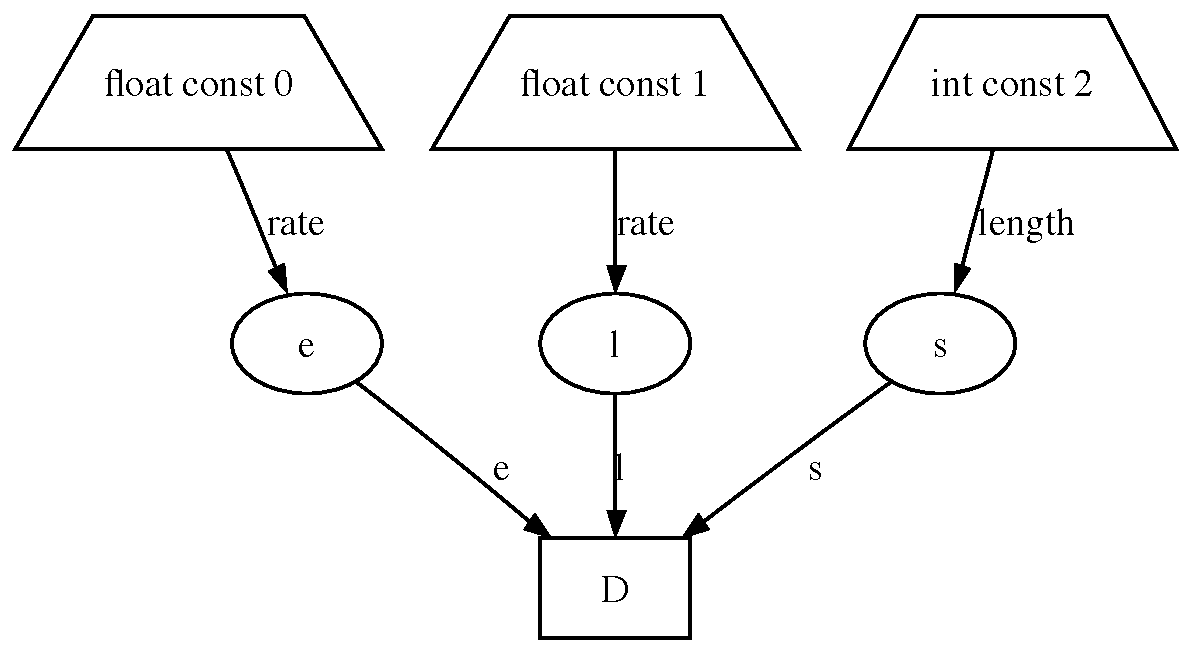
\epsfig{file=DisasterModel.pdf, width=6cm} 
\end{center} 
$D$ is shaded because it is flagged as data.

PyMC's symbol for functls is a downward-pointing triangle. A graphical representation of model \ref{disastermodel} with $r$ explicit follows:
\begin{center}
    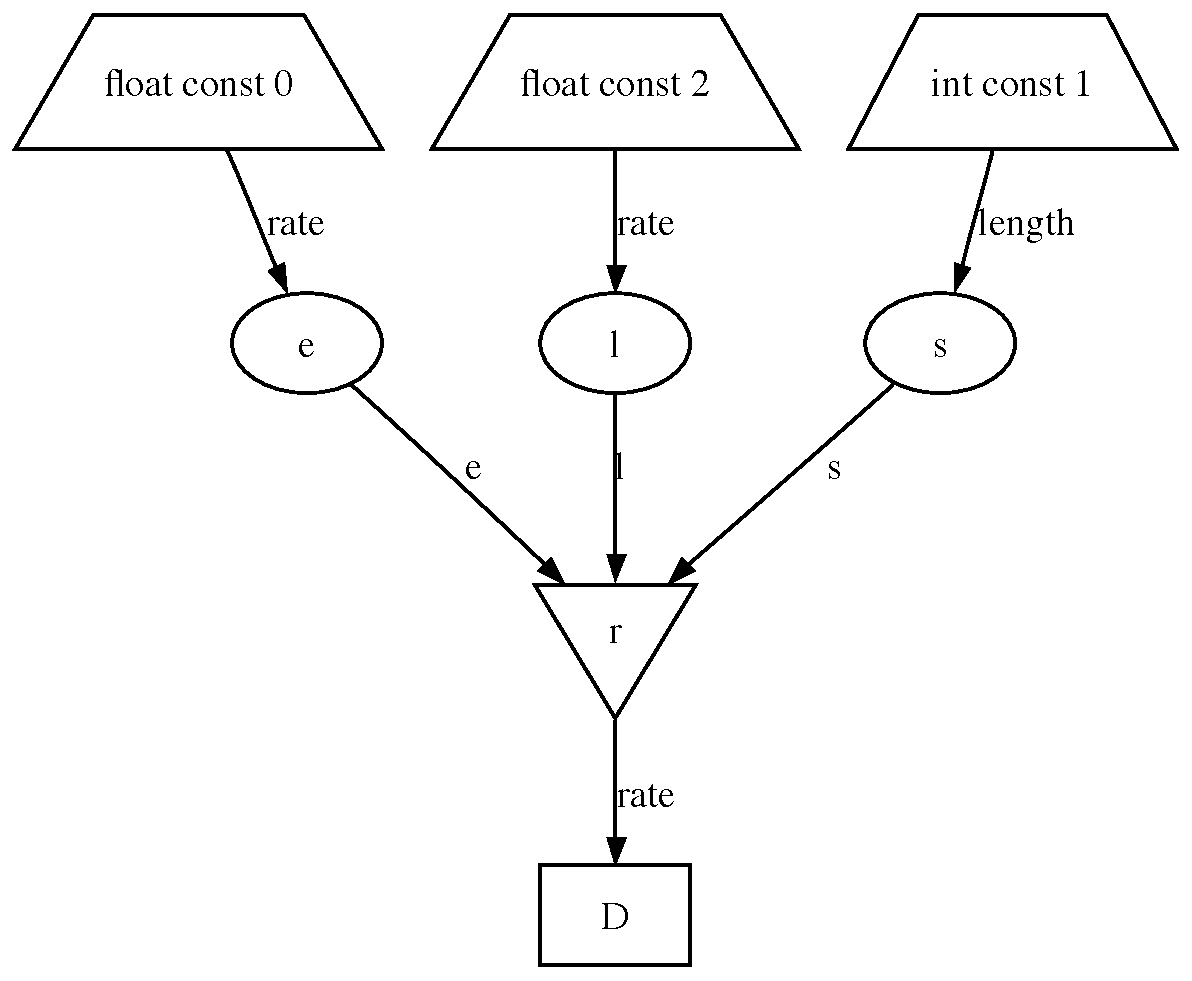
\epsfig{file=DisasterModel2.pdf, width=6cm} 
\end{center}
Note that if a functl has more than one child, its parents each inherit all of its children when it is made implicit:
\begin{center}
    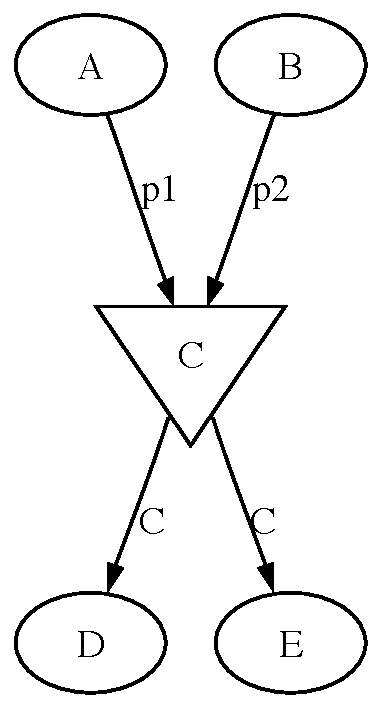
\epsfig{file=FunctionalPreInheritance.pdf, width=3.5cm} \textbf{XXX How can I move this arrow up?} $\Rightarrow$ 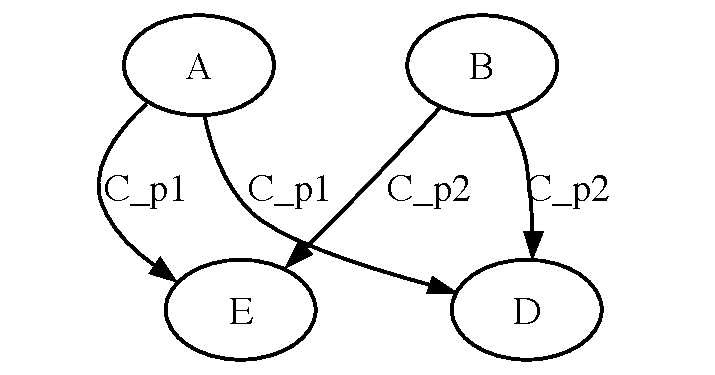
\epsfig{file=FunctionalPostInheritance.pdf, width=5cm}
\end{center}
Incidentally, these inherited children can be found using the function \texttt{extend\_children} provided by PyMC. Sampling method objects use this function to evaluate the log-likelihoods of the stochs they handle.

PyMC's symbol for potentials is a triple-outlined octagon:
\begin{center}
    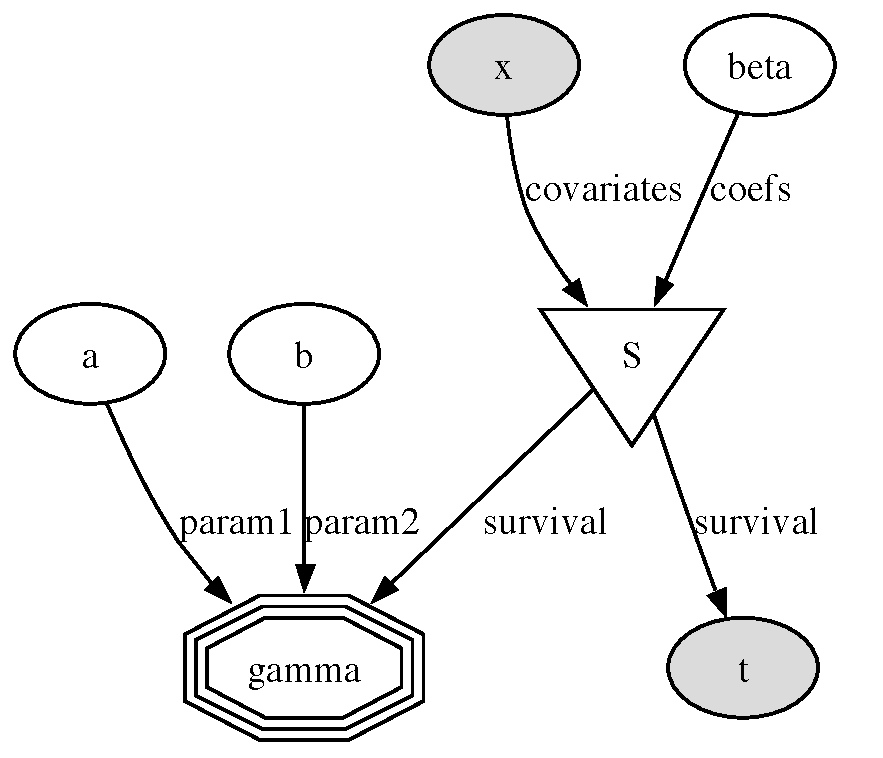
\epsfig{file=SurvivalModel.pdf, width=6cm} 
\end{center}
Potentials are usually associated with \emph{undirected} grahical models. In undirected representations, each parent of a potential is connected to every other parent by an undirected edge:
\begin{center}
    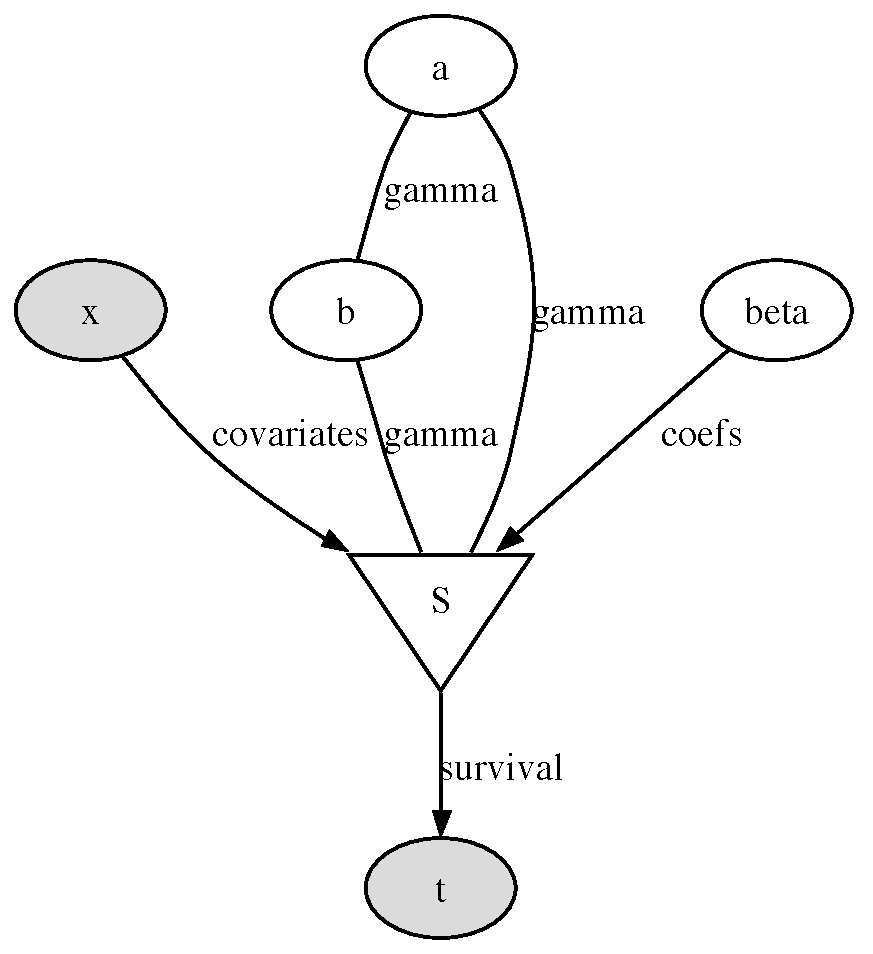
\epsfig{file=SurvivalModelCollapsed.pdf, width=5cm}
\end{center}
Mixing undirected and directed edges in the same model can be confusing, but fortunately the technique of \emph{moralization} can convert directed edges to undirected.

\cite{dawidmarkov} and \cite{jordangraphical} give several results on conditional independence and dependence that can be obtained just from looking at the structure of a graphical model, without knowing the forms of the probability distributions involved at all. A particularly important concept is $d$-separation, which determines when a group of stochs $A$ will be independent of another group $B$ given a third group $S$.

\section{Class \texttt{LazyFunction} and caching (optional)}

The \texttt{logp} attributes of stochs and potentials and the \texttt{value} attributes of functls are wrappers for instances of class \texttt{LazyFunction}. Lazy functions are wrappers for ordinary Python functions. A lazy function \texttt{L} could be instantiated from a function \texttt{fun} as follows:
\begin{verbatim}
L = LazyFunction(fun, arguments)
\end{verbatim}
The argument \texttt{arguments} is a dictionary; \texttt{fun} must accept keyword arguments only. When \texttt{L}'s \texttt{\bfseries get()} method is called, the return value is the same as the call 
\begin{verbatim}
fun(**argument_values)
\end{verbatim}
where the dictionary \texttt{argument\_values} is a copy of \texttt{arguments} in which each variable or container has been replaced by its \texttt{value} attribute. Note that no arguments need to be passed to \texttt{L.get}; lazy functions memorize their arguments.

Before calling \texttt{fun}, \texttt{L} will check the \texttt{argument\_values} dictionary against an internal cache. This comparison is done \emph{by reference}, not by value, and this is the reason why stochs' values cannot be updated in-place. If any of \texttt{argument\_values} is a container, the values of all the enclosed variables are checked against the internal cache. If each element of \texttt{argument\_values} matches a frame of the cache, the corresponding value is returned and \texttt{fun} is not called. If a call to \texttt{fun} is needed, \texttt{argument\_values} and the return value are added to the cache. The oldest frame in the cache is removed. The depth of the cache can be set using the optimal constructor argument \texttt{cache\_depth}, which defaults to 2.

Caching is helpful in MCMC, because variables' log-probabilities and values tend to be queried multiple times for the same parent configuration. The default cache depth of 2 turns out to be most useful in Metropolis-Hastings-type algorithms involving proposed values that may be rejected. To see why this is, write out an MCMC iteration for model (\ref{disastermodel}) using the Metropolis-Hastings algorithm, paying attention to the values of $D$'s parents when its log-probability is queried.

Lazy functions are implemented in C via Pyrex, and have been carefully optimized so that cache-checking does not actually slow down the simplest variables.


\section{The \texttt{Model} class} \label{sec:Model}
This class serves as a container for probability models and as a base class for the classes responsible for model fitting, like \texttt{Sampler}. Methods implemented:
\begin{description}
    \item[\texttt{sample\_model\_likelihood(\texttt{iter})}:] Returns \texttt{iter} samples from $\log p(d_M|\theta_M, M)$, the log-probability or log-density of all the data $d_M$ in model $M$ given all the stochs $\theta_M$. This is called by the function \texttt{weight()}, which finds the Bayes factors for a set of models.
    \item[\texttt{graph()}:] \textbf{XXX}
    \item[\texttt{tally()}:] Tells all stochs and functls to record their current values in their traces.
    \item[\texttt{remember(trace\_index)}:] Tells all stochs to revert to a certain index from their traces.
    \item[\texttt{status():}] \textbf{XXX}
    \item[\texttt{save\_traces(path, fname)}:] \textbf{XXX}
    \item[\texttt{seed()}:] \textbf{XXX}
\end{description}

Useful set attributes:
\begin{enumerate}
    \item \texttt{containers}
    \item \texttt{stochs}
    \item \texttt{functls}
    \item \texttt{variables}
    \item \texttt{potentials}
    \item \texttt{data}
\end{enumerate}



\subsection{Examples}\label{sub:example}
Here is the coal-mining disaster model implemented in PyMC with $r$ implicit, as in the left pane of figure \ref{fig:disasterdag}:
\begin{verbatim}
@stochastic
def s(value=50, length=110):
    """Change time for rate stoch."""
    constrain(value, 0, length)
    return 0.

@stochastic
def e(value=1., rate=1.):
    """Rate stoch of poisson distribution."""
    return exponential_like(value, rate)

@stochastic
def l(value=.1, rate = 1.):
    """Rate stoch of poisson distribution."""
    return exponential_like(value, rate)

@data
def D(  value = D_array,
        switchpoint = s,
        early_mean = e,
        late_mean = l):
    """Annual occurences of coal mining disasters."""
    return poisson_like(value[:s],e) + poisson_like(value[s:],l)
\end{verbatim}
To make $r$ explicit as in the right pane of figure \ref{fig:disasterdag}, we would write:
\begin{verbatim}
@stochastic
def s(value=50, length=110):
    """Change time for rate stoch."""
    constrain(value, 0, length)
    return 0.

@stochastic
def e(value=1., rate=1.):
    """Rate stoch of poisson distribution."""
    return exponential_like(value, rate)

@stochastic
def l(value=.1, rate = 1.):
    """Rate stoch of poisson distribution."""
    return exponential_like(value, rate)

@functional
def r(l=l,e=e,s=s):
    """r = function(l,e,s)"""
    ret_val =  ones(111,dtype=float)
    ret_val[:s] = e
    ret_val[s:] = l
    return ret_val

@data
def D(  value = D_array, rate=r):
    """Annual occurences of coal mining D."""
    return poisson_like(value,rate)
\end{verbatim}
In general, it's better to make heavyweight functions into their own functls, because functls' caches avoid unnecessary recomputation. In this case, however, the version with $r$ implicit is quite a bit faster.